\subsection{Elenco dei casi d'uso - Utente: sviluppatore}	

\subsubsection{UC-S1 Ricerca dei dati delle annotazioni}
		\begin{itemize}
			\item \textbf{Attori:} Sviluppatore.
			\item \textbf{Precondizione:} Lo sviluppatore si trova nell'area dati.
			\item \textbf{Postcondizione:} Lo sviluppatore ottiene una lista delle annotazioni correnti delle frasi.
			\item \textbf{Scenario principale:}
				\begin{enumerate}
					\item lo sviluppatore scrive nella barra di ricerca una sottostringa della frase cercata
					\item lo sviluppatore seleziona i filtri da usare nella ricerca (UC-S1.1)
					\item lo sviluppatore conferma la ricerca
					\item lo sviluppatore visualizza le annotazioni filtrate (UC-S1.2)
				\end{enumerate}
		\end{itemize}
	
	\subsubsection{UC-S1.1 Filtraggio dei dati}	
		\begin{itemize}
			\item \textbf{Attori:} Sviluppatore.
			\item \textbf{Precondizione:} Lo sviluppatore si trova nell'area dati e ha scritto nella barra di ricerca una sottostringa della frase cercata.
			\item \textbf{Postcondizione:} Lo sviluppatore ha indicato i filtri da applicare alla ricerca.
			\item \textbf{Scenario principale:}
				\begin{enumerate}
					\item lo sviluppatore seleziona il filtro su base temporale (UC-S1.1.1)
					\item lo sviluppatore seleziona il filtro in base agli utenti (UC-S1.1.2)
				\end{enumerate}
			\end{itemize}
	\begin{figure}[h]
			\centering
			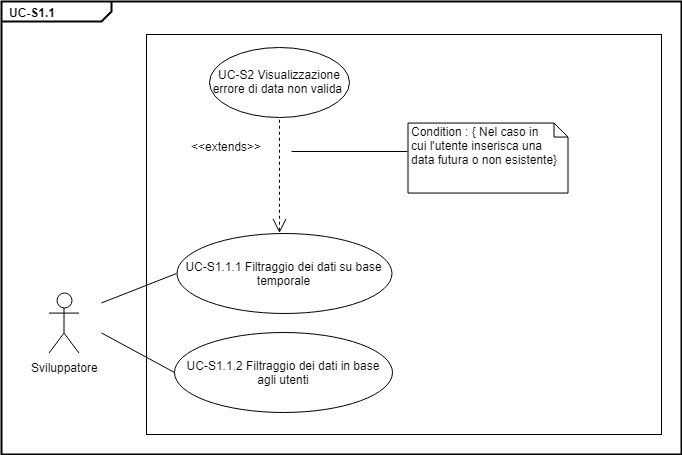
\includegraphics[scale=0.7]{images/UC-S1_1.png}
			\caption{UC-S1.1 Filtraggio dei dati}
		\end{figure}	

	\subsubsection{UC-S1.2 Visualizzazione dell'annotazione in lista}
		\begin{itemize}
			\item \textbf{Attori:} Sviluppatore.
			\item \textbf{Precondizione:} Lo sviluppatore si trova nell'area dati.
			\item \textbf{Postcondizione:} Lo sviluppatore visualizza le informazioni di un'annotazione.
			\item \textbf{Scenario principale:}
				\begin{enumerate}
					\item lo sviluppatore visualizza la data dell'annotazione
					\item lo sviluppatore visualizza l'username dell'utente autore dell'annotazione
					\item lo sviluppatore visualizza l'ID dell'esercizio
				\end{enumerate}
		\end{itemize}
		
	\subsubsection{UC-S1.1.1 Filtraggio dei dati su base temporale}	
		\begin{itemize}
			\item \textbf{Attori:} Sviluppatore.
			\item \textbf{Precondizione:} Lo sviluppatore si trova nell'area dati e ha scritto nella barra di ricerca una sottostringa della frase cercata.
			\item \textbf{Postcondizione:} Lo sviluppatore ha indicato il filtro su base temporale della ricerca.
			\item \textbf{Scenario principale:}
				\begin{enumerate}
					\item lo sviluppatore indica due date che definiscono un intervallo di tempo per restringere la ricerca
				\end{enumerate}
			\item \textbf{Estensioni:}
				\begin{itemize}
					\item 1.a Se i parametri inseriti dall'utente non sono coerenti viene mostrato un messaggio di errore (UC-S2).
				\end{itemize}		
		\end{itemize}

	\subsubsection{UC-S1.1.2 Filtraggio dei dati in base agli utenti}	
		\begin{itemize}
			\item \textbf{Attori:} Sviluppatore.
			\item \textbf{Precondizione:} Lo sviluppatore si trova nell'area dati e ha scritto nella barra di ricerca una sottostringa della frase cercata.
			\item \textbf{Postcondizione:} Lo sviluppatore ha indicato il filtro in base agli utenti.
			\item \textbf{Scenario principale:}
				\begin{enumerate}
					\item lo sviluppatore sceglie tra le opzioni "Includi utente"
					\item lo sviluppatore cerca gli utenti da includere (UC-S1.1.2.1)
					\item lo sviluppatore indica gli utenti da includere
				\end{enumerate}
		\end{itemize}
		
	\subsubsection{UC-S1.1.2.1 Ricerca utente}
		\begin{itemize}
			\item \textbf{Attori:} Sviluppatore.
			\item \textbf{Precondizione:} Lo sviluppatore ha scelto di includere un utente.
			\item \textbf{Postcondizione:} Lo sviluppatore visualizza una lista di username contenenti la stringa inserita.
			\item \textbf{Scenario principale:}
			\begin{enumerate}
				\item lo sviluppatore scrive l'username di un utente, o una sua parte
			\end{enumerate}
		\end{itemize}		
			
	\subsubsection{UC-S1.1.3 Filtraggio dei dati in base al ruolo}	
		\begin{itemize}
			\item \textbf{Attori:} Sviluppatore.
			\item \textbf{Precondizione:} Lo sviluppatore si trova nell'area dati e ha scritto nella barra di ricerca una sottostringa della frase cercata.
			\item \textbf{Postcondizione:} Lo sviluppatore ha indicato il filtro in base al ruolo.
			\item \textbf{Scenario principale:}
				\begin{enumerate}
					\item lo sviluppatore indica un ruolo tra "Insegnante" e " Studente"
				\end{enumerate}
		\end{itemize}

	\subsubsection{UC-S1.1.4 Filtraggio dei dati in base alla valutazione}	
		\begin{itemize}
			\item \textbf{Attori:} Sviluppatore.
			\item \textbf{Precondizione:} Lo sviluppatore si trova nell'area dati e ha scritto nella barra di ricerca una sottostringa della frase cercata.
			\item \textbf{Postcondizione:} Lo sviluppatore ha indicato il filtro in base alla valutazione.
			\item \textbf{Scenario principale:}
				\begin{enumerate}
					\item lo sviluppatore indica due numeri (da 0 a 10) che definiscono un intervallo di voti per restringere la ricerca
				\end{enumerate}
			\item \textbf{Estensioni:}
				\begin{itemize}
					\item 1.a Se i parametri inseriti dall'utente non sono coerenti viene mostrato un messaggio di errore (UC-S18).
				\end{itemize}
		\end{itemize}	
	
	\subsubsection{UC-S2 Visualizzazione errore di data non valida}
		\begin{itemize}					
			\item \textbf{Attori:} Sviluppatore.
			\item \textbf{Precondizione:} Lo sviluppatore ha indicato un intervallo di tempo non valido.
			\item \textbf{Postcondizione:} Lo sviluppatore torna all'area dati.
			\item \textbf{Scenario principale:}
				\begin{enumerate}
					\item lo sviluppatore visualizza un messaggio di errore "L'intervallo di tempo indicato non è valido"
				\end{enumerate}
		\end{itemize}
			
	\subsubsection{UC-S3 Visualizzazione dei dati di una annotazione di una frase}
		\begin{itemize}
			\item \textbf{Attori:} Sviluppatore.
			\item \textbf{Precondizione:} Lo sviluppatore visualizza la lista delle annotazioni ricercate.
			\item \textbf{Postcondizione:} Lo sviluppatore legge i dati di una annotazione di una frase.
			\item \textbf{Scenario principale:}
				\begin{enumerate}
					\item lo sviluppatore seleziona una annotazione
					\item lo sviluppatore visualizza data, utente, ID esercizio e soluzione proposta
				\end{enumerate}
		\end{itemize}
	
	\subsubsection{UC-S4 Visualizzazione storico}		
		\begin{itemize}
			\item \textbf{Attori:} Sviluppatore.
			\item \textbf{Precondizione:} Lo sviluppatore visualizza la lista delle annotazioni ricercate.
			\item \textbf{Postcondizione:} Lo sviluppatore visualizza lo storico delle annotazioni ottenute dalla ricerca precedente.
			\item \textbf{Scenario principale:}
			\begin{enumerate}
				\item lo sviluppatore seleziona l'opzione "vedi storico"
			\end{enumerate}
		\end{itemize}	
		
	\subsubsection{UC-S5 Ordinamento dei risultati}
		\begin{itemize}
			\item \textbf{Attori:} Sviluppatore.
			\item \textbf{Precondizione:} Lo sviluppatore visualizza la lista delle annotazioni ricercate.
			\item \textbf{Postcondizione:} Lo sviluppatore ottiene la lista precedente ordinata in base alle scelte effettuate.
			\item \textbf{Scenario principale:}
				\begin{enumerate}
					\item lo sviluppatore sceglie il parametro secondo il quale ordinare i risultati (alfabetico, frequenza, ultima correzione, utente).
					\item lo sviluppatore conferma l'ordinamento scelto.
				\end{enumerate}
		\end{itemize} 
	
	\subsubsection{UC-S6 Download dei dati raccolti}
		\begin{itemize}
			\item \textbf{Attori:} Sviluppatore.
			\item \textbf{Precondizione:} Lo sviluppatore visualizza la lista delle annotazioni ricercate.
			\item \textbf{Postcondizione:} Lo sviluppatore ottiene un file con i dati dei risultati precedentemente trovati.
			\item \textbf{Scenario principale:}
				\begin{enumerate}
					\item lo sviluppatore richiede il download dei dati
					\item lo sviluppatore decide il path in cui il file viene salvato
					\item lo sviluppatore sceglie il formato dei dati da scaricare
					\item lo sviluppatore esegue il salvataggio
				\end{enumerate}
		\end{itemize}	
		
		\begin{figure}[h]
		\centering
		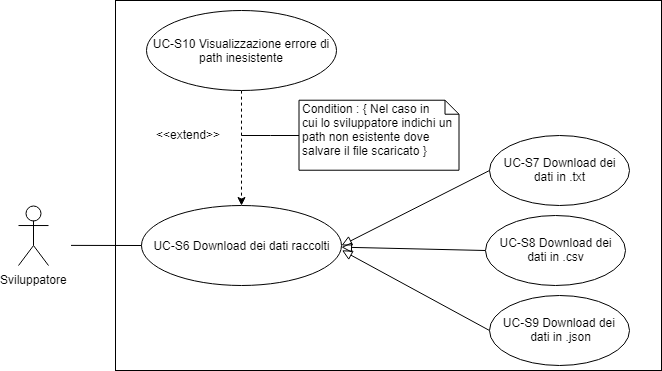
\includegraphics[scale=0.7]{images/UC-S6.png}
		\caption{UC-S6 Download dei dati raccolti}
	\end{figure}
	
\subsubsection{UC-S7 Download dei dati raccolti in \texttt{.txt}}
		\begin{itemize}
			\item \textbf{Attori:} Sviluppatore.
			\item \textbf{Precondizione:} Lo sviluppatore visualizza la lista delle annotazioni ricercate.
			\item \textbf{Postcondizione:} Lo sviluppatore ottiene un file con i dati dei risultati precedentemente trovati in formato \texttt{.txt}.
			\item \textbf{Scenario principale:}
				\begin{enumerate}
					\item lo sviluppatore richiede il download dei dati
					\item lo sviluppatore decide il path in cui il file viene salvato
					\item lo sviluppatore sceglie il formato \texttt{.txt} per il download dei dati
					\item lo sviluppatore esegue il salvataggio
				\end{enumerate}
		\end{itemize}

\subsubsection{UC-S8 Download dei dati raccolti in \texttt{.csv}}
		\begin{itemize}
			\item \textbf{Attori:} Sviluppatore.
			\item \textbf{Precondizione:} Lo sviluppatore visualizza la lista delle annotazioni ricercate.
			\item \textbf{Postcondizione:} Lo sviluppatore ottiene un file con i dati dei risultati precedentemente trovati in formato \texttt{.csv}.
			\item \textbf{Scenario principale:}
				\begin{enumerate}
					\item lo sviluppatore richiede il download dei dati
					\item lo sviluppatore decide il path in cui il file viene salvato
					\item lo sviluppatore sceglie il formato \texttt{.csv} per il download dei dati
					\item lo sviluppatore esegue il salvataggio
				\end{enumerate}
		\end{itemize}

\subsubsection{UC-S9 Download dei dati raccolti in \texttt{.json}}
		\begin{itemize}
			\item \textbf{Attori:} Sviluppatore.
			\item \textbf{Precondizione:} Lo sviluppatore visualizza la lista delle annotazioni ricercate.
			\item \textbf{Postcondizione:} Lo sviluppatore ottiene un file con i dati dei risultati precedentemente trovati in formato \texttt{.json}.
			\item \textbf{Scenario principale:}
				\begin{enumerate}
					\item lo sviluppatore richiede il download dei dati
					\item lo sviluppatore decide il path in cui il file viene salvato
					\item lo sviluppatore sceglie il formato \texttt{.json} per il download dei dati
					\item lo sviluppatore esegue il salvataggio
				\end{enumerate}
		\end{itemize}
				
	\subsubsection{UC-S11 Download di un dataset}
		\begin{itemize}
			\item \textbf{Attori:} Sviluppatore.
			\item \textbf{Precondizione:} Lo sviluppatore visualizza la lista delle annotazioni ricercate.
			\item \textbf{Postcondizione:} Lo sviluppatore ottiene il dataset in un file \texttt{.txt}.
			\item \textbf{Scenario principale:}
			\begin{enumerate}
				\item lo sviluppatore richiede il download del dataset, contenente l'input della fase di train del software di apprendimento automatico in base alla ricerca effettuata
				\item lo sviluppatore decide il path in cui il file viene salvato
				\item lo sviluppatore esegue il salvataggio
			\end{enumerate}
		\end{itemize}
		
	\subsubsection{UC-S12 Visualizzazione lista dei modelli}
		\begin{itemize}
			\item \textbf{Attori:} Sviluppatore.
			\item \textbf{Precondizione:} Lo sviluppatore si trova nell'area dati.
			\item \textbf{Postcondizione:} Lo sviluppatore visualizza la lista dei modelli disponibili per l'applicazione.
			\item \textbf{Scenario principale:}
			\begin{enumerate}
					\item lo sviluppatore seleziona la voce "Lista dei modelli"
					\item lo sviluppatore visualizza i modelli (UC-S12.1)
				\end{enumerate}
		\end{itemize}	
		
\subsubsection{UC-S12.1 Visualizzazione modello in lista}
		\begin{itemize}
			\item \textbf{Attori:} Sviluppatore.
			\item \textbf{Precondizione:} Lo sviluppatore si trova nell'area dati.
			\item \textbf{Postcondizione:} Lo sviluppatore visualizza le informazioni riguardanti un modello.
			\item \textbf{Scenario principale:}
			\begin{enumerate}
					\item lo sviluppatore visualizza il nome del modello
					\item lo sviluppatore visualizza la lingua del modello
				\end{enumerate}
		\end{itemize}			
	
	\subsubsection{UC-S13 Download di un modello}
		\begin{itemize}
			\item \textbf{Attori:} Sviluppatore.
			\item \textbf{Precondizione:} Lo sviluppatore visualizza la lista dei modelli disponibili per l'applicazione.
			\item \textbf{Postcondizione:} Lo sviluppatore ottiene un file binario con il modello.
			\item \textbf{Scenario principale:}
			\begin{enumerate}
				\item lo sviluppatore seleziona un modello
				\item lo sviluppatore seleziona l'opzione "Download"
				\item lo sviluppatore decide il path in cui il file viene salvato
				\item lo sviluppatore esegue il salvataggio
			\end{enumerate}
		\end{itemize}	
		
		\begin{figure}[h]
		\centering
		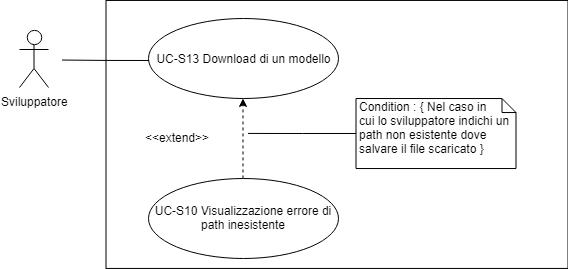
\includegraphics[scale=0.7]{images/UC-S13.png}
		\caption{UC-S13 Download di un modello}
		\end{figure}

	\subsubsection{UC-S14 Visualizzazione informazioni di un modello}
		\begin{itemize}
			\item \textbf{Attori:} Sviluppatore.
			\item \textbf{Precondizione:} Lo sviluppatore visualizza la lista dei modelli disponibili per l'applicazione.
			\item \textbf{Postcondizione:} Lo sviluppatore visualizza le informazioni di un modello (nome, data creazione, periodo di utilizzo, lingua).
			\item \textbf{Scenario principale:}
			\begin{enumerate}
				\item lo sviluppatore seleziona un modello
				\item lo sviluppatore seleziona l'opzione "Visualizza informazioni"
				\end{enumerate}
		\end{itemize}
		
	\subsubsection{UC-S15 Creazione di un modello}		
		\begin{itemize}
			\item \textbf{Attori:} Sviluppatore.
			\item \textbf{Precondizione:} Lo sviluppatore si trova nell'area dati.
			\item \textbf{Postcondizione:} Lo sviluppatore ha aggiunto un modello alla piattaforma.
			\item \textbf{Scenario principale:}
			\begin{enumerate}
				\item lo sviluppatore seleziona la voce "Aggiungi modello"
				\item lo sviluppatore inserisce un file che contiene un dataset
				\item lo sviluppatore conferma la creazione
			\end{enumerate}
			\item \textbf{Estensioni:}
				\begin{itemize}
					\item 2.a Se il dataset fornito ha un formato errato, viene visualizzato un messaggio di errore (UC-S16).
				\end{itemize}
		\end{itemize}
		
		\begin{figure}[h]
			\centering
			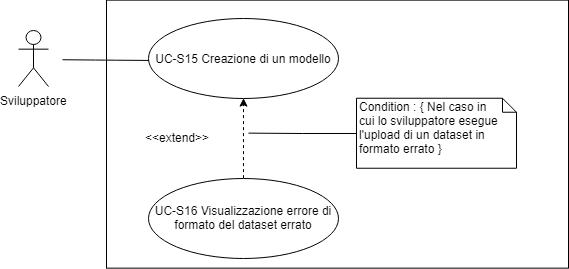
\includegraphics[scale=0.7]{images/UC-S15.png}
				\caption{UC-S15 Creazione di un modello}
		\end{figure}	
	
	\subsubsection{UC-S16 Visualizzazione errore di formato del dataset errato}	
	\begin{itemize}					
			\item \textbf{Attori:} Sviluppatore.
			\item \textbf{Precondizione:} Lo sviluppatore ha fornito un dataset con un formato non corretto.
			\item \textbf{Postcondizione:} Lo sviluppatore torna all'area dati.
			\item \textbf{Scenario principale:}
				\begin{enumerate}
					\item lo sviluppatore visualizza un messaggio di errore "Formato dataset non corretto"
				\end{enumerate}	
		\end{itemize}		
	
	\subsubsection{UC-S17 Cambio modello}
	\begin{itemize}					
			\item \textbf{Attori:} Sviluppatore.
			\item \textbf{Precondizione:} Lo sviluppatore visualizza la lista dei modelli disponibili per l'applicazione.
			\item \textbf{Postcondizione:} Lo sviluppatore ha cambiato il modello utilizzato dal software di apprendimento automatico.
			\item \textbf{Scenario principale:}
				\begin{enumerate}
					\item lo sviluppatore seleziona il modello che vuole utilizzare da una lista di modelli caricati o creati precedentemente
					\item lo sviluppatore seleziona l'opzione "Usa questo modello"
					\item lo sviluppatore conferma le modifiche
				\end{enumerate}	
		\end{itemize}		
	
	\subsubsection{UC-S18 Visualizzazione errore di valutazioni non valide}
		\begin{itemize}					
			\item \textbf{Attori:} Sviluppatore.
			\item \textbf{Precondizione:} Lo sviluppatore ha indicato un intervallo di voti non valido.
			\item \textbf{Postcondizione:} Lo sviluppatore torna all'area dati.
			\item \textbf{Scenario principale:}
				\begin{enumerate}
					\item lo sviluppatore visualizza un messaggio di errore "L'intervallo di voti indicato non è valido"
				\end{enumerate}
		\end{itemize}